% --- Page Style ---
\settasks{label-width=4.6em, item-indent=4.6em}
\pagestyle{fancy}
\fancyhf{}
\lhead{Algebra --- Unit 8}
\rhead{Exam ID: \underline{\hspace{2cm}}}
\lfoot{Show all work. Round to nearest thousandth unless stated.}
\rfoot{Page \thepage}
\renewcommand{\headrulewidth}{0.4pt}
\renewcommand{\footrulewidth}{0.4pt}

% --- Header spanning both columns ---
\twocolumn[
  \begin{center}
    {\huge \textbf{Unit 8 Test}} \\
    \vgap
    {\large \textbf{Algebra}} \\
    \vgap
    \begin{tabular}{|l|l|}
      \hline
      \textbf{Student Name:} & \hspace{6cm} \\ \hline
      \textbf{Date:} & \hspace{6cm} \\ \hline
    \end{tabular}
  \end{center}
  \vgap
  \textbf{Instructions:} Show all necessary work. If no triangle exists, write ``DNE'' and explain.
  \vgap
]

% % --- Form A ---
% \section*{Form A}

% \begin{enumerate}[leftmargin=*, label=\textbf{\arabic*.}]

%   \item Find $BC$ in the triangle shown below. Round to the nearest thousandth. \points{2}

%   \begin{center}
%   \begin{tikzpicture}[scale=0.9, line cap=round, line join=round]
%     \draw[thick] (0,0) node[left] {$B$} -- (4,0) node[right] {$C$} -- (2.2,2.8) node[above] {$A$} -- cycle;
%     \node[below] at (2,0) {$12$};
%     \node[above right] at (3.1,1.4) {$9$};
%     \node[below left] at (1.1,1.4) {$28^{\circ}$};
%   \end{tikzpicture}
%   \end{center}

%   $BC = $ \blank
%   \vgapp

%   \item Find $m\angle A$ in the triangle shown below. Round to the nearest thousandth. \points{2}

%   \begin{center}
%   \begin{tikzpicture}[scale=0.9, line cap=round, line join=round]
%     \draw[thick] (0,0) node[left] {$B$} -- (5,0) node[right] {$C$} -- (1.8,2.2) node[above] {$A$} -- cycle;
%     \node[below] at (2.5,0) {$14$};
%     \node[above right] at (3.4,1.1) {$11$};
%     \node[above left] at (0.9,1.1) {$7$};
%   \end{tikzpicture}
%   \end{center}

%   $m\angle A = $ \blank
%   \vgapp

%   \item Triangle $ABC$ has $m\angle C = 38^{\circ}$, $b = 27$, $c = 12$. Find all sides and angles. If no solution exists, write DNE and explain. \points{3}

%   $a = $ \blank

%   $b = $ \blank

%   $c = $ \blank

%   $m\angle A = $ \blank

%   $m\angle B = $ \blank

%   $m\angle C = $ \blank
%   \vgappp

%   \item Triangle $ABC$ has $m\angle B = 51^{\circ}$, $a = 31$, $b = 28$. Find all sides and angles. If no solution exists, write DNE and explain. \points{3}

%   $a = $ \blank

%   $b = $ \blank

%   $c = $ \blank

%   $m\angle A = $ \blank

%   $m\angle B = $ \blank

%   $m\angle C = $ \blank
%   \vgappp

%   \item Triangle $ABC$ has $m\angle B = 41^{\circ}$, $a = 35$, $c = 22$. Find all sides and angles. If no solution exists, write DNE and explain. \points{3}

%   $a = $ \blank

%   $b = $ \blank

%   $c = $ \blank

%   $m\angle A = $ \blank

%   $m\angle B = $ \blank

%   $m\angle C = $ \blank
%   \vgappp

%   \item A triangle has side lengths 4, 10, and 13. Find the area. Round to the nearest thousandth. \points{3}
%   \vgappp

%   \item A rock climber sees the peak of Gray Mountain at an angle of elevation of $33^{\circ}$ and the base at an angle of depression of $39^{\circ}$. Gray Mountain is 3072 feet high and the base is at sea level. What is the climber's elevation to the nearest inch? \points{4}
%   \vgappp

%   \item Gina's phone works within 45 miles of the tower. She drives 36 miles past the tower on Hwy 7, then 25 miles on Oakville Road to Piggly Wiggly. Is she within range? Explain. \points{3}
%   \vgappp

%   \item A ship leaves Port Sarim at 9:00 AM Wednesday for Entrana, 700 miles at bearing $35^{\circ}$ E of N. To avoid a kraken cove, they sail north 12 hours at 35 mph. \points{4}

%   \begin{tasks}(1)
%     \task At what angle should they turn to head directly to Entrana? \blank
%     \task At what time (nearest minute) will they arrive? \blank
%   \end{tasks}
%   \vgappp

%   \item The chicken claims a triangle $ABC$ exists with $AB = 24$ in, $BC = 18$ in, and $m\angle A = \dfrac{2\pi}{9}$ radians. The egg says it is impossible. Who is correct? Explain. \points{3}
%   \vgappp

% \end{enumerate}

% \clearpage
% % --- Form B ---
% \section*{Form B}

% \begin{enumerate}[leftmargin=*, label=\textbf{\arabic*.}, resume]

%   \item Find $BC$ in the triangle shown below. Round to the nearest thousandth. \points{2}

%   \begin{center}
%   \begin{tikzpicture}[scale=0.9, line cap=round, line join=round]
%     \draw[thick] (0,0) node[left] {$B$} -- (4.2,0) node[right] {$C$} -- (2,2.6) node[above] {$A$} -- cycle;
%     \node[below] at (2.1,0) {$13$};
%     \node[above right] at (3.1,1.3) {$10$};
%     \node[below left] at (1,1.3) {$32^{\circ}$};
%   \end{tikzpicture}
%   \end{center}

%   $BC = $ \blank
%   \vgapp

%   \item Find $m\angle A$ in the triangle shown below. Round to the nearest thousandth. \points{2}

%   \begin{center}
%   \begin{tikzpicture}[scale=0.9, line cap=round, line join=round]
%     \draw[thick] (0,0) node[left] {$B$} -- (5,0) node[right] {$C$} -- (2,2.4) node[above] {$A$} -- cycle;
%     \node[below] at (2.5,0) {$15$};
%     \node[above right] at (3.5,1.2) {$12$};
%     \node[above left] at (1,1.2) {$8$};
%   \end{tikzpicture}
%   \end{center}

%   $m\angle A = $ \blank
%   \vgapp

%   \item Triangle $ABC$ has $m\angle C = 58^{\circ}$, $b = 33$, $c = 29$. Find all sides and angles. If no solution exists, write DNE and explain. \points{3}

%   $a = $ \blank

%   $b = $ \blank

%   $c = $ \blank

%   $m\angle A = $ \blank

%   $m\angle B = $ \blank

%   $m\angle C = $ \blank
%   \vgappp

%   \item Triangle $ABC$ has $m\angle B = 31^{\circ}$, $a = 39$, $b = 17$. Find all sides and angles. If no solution exists, write DNE and explain. \points{3}

%   $a = $ \blank

%   $b = $ \blank

%   $c = $ \blank

%   $m\angle A = $ \blank

%   $m\angle B = $ \blank

%   $m\angle C = $ \blank
%   \vgappp

%   \item Triangle $ABC$ has $m\angle B = 61^{\circ}$, $a = 31$, $c = 26$. Find all sides and angles. If no solution exists, write DNE and explain. \points{3}

%   $a = $ \blank

%   $b = $ \blank

%   $c = $ \blank

%   $m\angle A = $ \blank

%   $m\angle B = $ \blank

%   $m\angle C = $ \blank
%   \vgappp

%   \item A triangle has side lengths 7, 9, and 11. Find the area. Round to the nearest thousandth. \points{3}
%   \vgappp

%   \item A rock climber sees the peak of Gray Mountain at an angle of elevation of $30^{\circ}$ and the base at an angle of depression of $41^{\circ}$. Gray Mountain is 3072 feet high and the base is at sea level. What is the climber's elevation to the nearest inch? \points{4}
%   \vgappp

%   \item Gina's phone works within 50 miles of the tower. She drives 36 miles past the tower on Hwy 7, then 25 miles on Oakville Road to Piggly Wiggly. Is she within range? Explain. \points{3}
%   \vgappp

%   \item A ship leaves Port Sarim at 9:00 AM Wednesday for Entrana, 650 miles at bearing $35^{\circ}$ N of W. To avoid a kraken cove, they sail west 12 hours at 40 mph. \points{4}

%   \begin{tasks}(1)
%     \task At what angle should they turn to head directly to Entrana? \blank
%     \task At what time (nearest minute) will they arrive? \blank
%   \end{tasks}
%   \vgappp

%   \item The chicken claims a triangle $ABC$ exists with $AB = 24$ in, $BC = 19$ in, and $m\angle A = \dfrac{5\pi}{18}$ radians. The egg says it is impossible. Who is correct? Explain. \points{3}
%   \vgappp

% \end{enumerate}

% \clearpage
% % --- Form C ---
% \section*{Form C}

% \begin{enumerate}[leftmargin=*, label=\textbf{\arabic*.}, resume]

%   \item Find $BC$ in the triangle shown below. Round to the nearest thousandth. \points{2}

%   \begin{center}
%   \begin{tikzpicture}[scale=0.9, line cap=round, line join=round]
%     \draw[thick] (0,0) node[left] {$B$} -- (3.8,0) node[right] {$C$} -- (2.2,2.4) node[above] {$A$} -- cycle;
%     \node[below] at (1.9,0) {$11$};
%     \node[above right] at (3,1.2) {$8$};
%     \node[below left] at (1.1,1.2) {$36^{\circ}$};
%   \end{tikzpicture}
%   \end{center}

%   $BC = $ \blank
%   \vgapp

%   \item Find $m\angle A$ in the triangle shown below. Round to the nearest thousandth. \points{2}

%   \begin{center}
%   \begin{tikzpicture}[scale=0.9, line cap=round, line join=round]
%     \draw[thick] (0,0) node[left] {$B$} -- (4.5,0) node[right] {$C$} -- (1.6,2.2) node[above] {$A$} -- cycle;
%     \node[below] at (2.25,0) {$13$};
%     \node[above right] at (3,1.1) {$10$};
%     \node[above left] at (0.8,1.1) {$6$};
%   \end{tikzpicture}
%   \end{center}

%   $m\angle A = $ \blank
%   \vgapp

%   \item Triangle $ABC$ has $m\angle C = 52^{\circ}$, $b = 19$, $c = 13$. Find all sides and angles. If no solution exists, write DNE and explain. \points{3}

%   $a = $ \blank

%   $b = $ \blank

%   $c = $ \blank

%   $m\angle A = $ \blank

%   $m\angle B = $ \blank

%   $m\angle C = $ \blank
%   \vgappp

%   \item Triangle $ABC$ has $m\angle B = 36^{\circ}$, $a = 37$, $b = 24$. Find all sides and angles. If no solution exists, write DNE and explain. \points{3}

%   $a = $ \blank

%   $b = $ \blank

%   $c = $ \blank

%   $m\angle A = $ \blank

%   $m\angle B = $ \blank

%   $m\angle C = $ \blank
%   \vgappp

%   \item Triangle $ABC$ has $m\angle B = 41^{\circ}$, $a = 29$, $c = 16$. Find all sides and angles. If no solution exists, write DNE and explain. \points{3}

%   $a = $ \blank

%   $b = $ \blank

%   $c = $ \blank

%   $m\angle A = $ \blank

%   $m\angle B = $ \blank

%   $m\angle C = $ \blank
%   \vgappp

%   \item A triangle has side lengths 7, 11, and 14. Find the area. Round to the nearest thousandth. \points{3}
%   \vgappp

%   \item A rock climber sees the peak of Gray Mountain at an angle of elevation of $31^{\circ}$ and the base at an angle of depression of $38^{\circ}$. Gray Mountain is 4081 feet high and the base is at sea level. What is the climber's elevation to the nearest inch? \points{4}
%   \vgappp

%   \item Gina's phone works within 50 miles of the tower. She drives 36 miles past the tower on Hwy 7, then 30 miles on Oakville Road to Piggly Wiggly. Is she within range? Explain. \points{3}
%   \vgappp

%   \item A ship leaves Port Sarim at 9:00 AM Wednesday for Entrana, 750 miles at bearing $35^{\circ}$ W of N. To avoid a kraken cove, they sail north 10 hours at 40 mph. \points{4}

%   \begin{tasks}(1)
%     \task At what angle should they turn to head directly to Entrana? \blank
%     \task At what time (nearest minute) will they arrive? \blank
%   \end{tasks}
%   \vgappp

%   \item The chicken claims a triangle $ABC$ exists with $AB = 31$ in, $BC = 18$ in, and $m\angle A = \dfrac{\pi}{5}$ radians. The egg says it is impossible. Who is correct? Explain. \points{3}
%   \vgappp

% \end{enumerate}

% \clearpage
% % --- Form D ---
% \section*{Form D}

\begin{enumerate}[leftmargin=*, label=\textbf{\arabic*.}, resume]

  \item Find $BC$ in the triangle shown below. Round to the nearest thousandth. \points{2}

  \begin{center}
  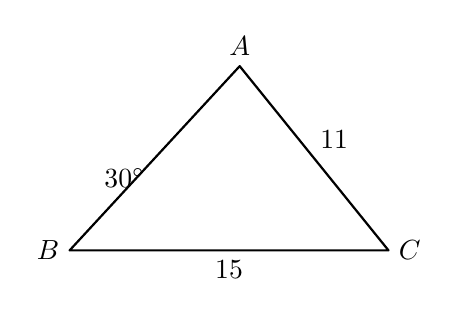
\begin{tikzpicture}[scale=0.9, line cap=round, line join=round]
    \draw[thick] (0,0) node[left] {$B$} -- (4.5,0) node[right] {$C$} -- (2.4,2.6) node[above] {$A$} -- cycle;
    \node[below] at (2.25,0) {$15$};
    \node[above right] at (3.4,1.3) {$11$};
    \node[below left] at (1.2,1.3) {$30^{\circ}$};
  \end{tikzpicture}
  \end{center}

  $BC = $ \blank
  \vgapp

  \item Find $m\angle A$ in the triangle shown below. Round to the nearest thousandth. \points{2}

  \begin{center}
  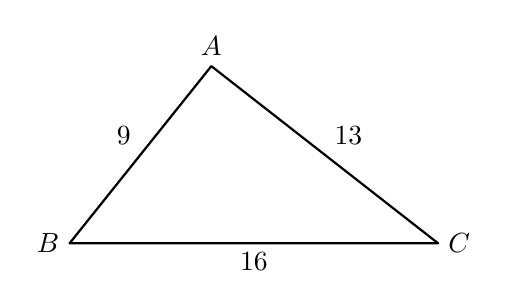
\begin{tikzpicture}[scale=0.9, line cap=round, line join=round]
    \draw[thick] (0,0) node[left] {$B$} -- (5.2,0) node[right] {$C$} -- (2,2.5) node[above] {$A$} -- cycle;
    \node[below] at (2.6,0) {$16$};
    \node[above right] at (3.6,1.25) {$13$};
    \node[above left] at (1,1.25) {$9$};
  \end{tikzpicture}
  \end{center}

  $m\angle A = $ \blank
  \vgapp



  \newpage
  \item Triangle $ABC$ has $m\angle C = 44^{\circ}$, $b = 25$, $c = 14$. Find all sides and angles. If no solution exists, write DNE and explain. \points{3}

  $a = $ \blank

  $b = $ \blank

  $c = $ \blank

  $m\angle A = $ \blank

  $m\angle B = $ \blank

  $m\angle C = $ \blank
  \vgappp

  \item Triangle $ABC$ has $m\angle B = 47^{\circ}$, $a = 28$, $b = 22$. Find all sides and angles. If no solution exists, write DNE and explain. \points{3}

  $a = $ \blank

  $b = $ \blank

  $c = $ \blank

  $m\angle A = $ \blank

  $m\angle B = $ \blank

  $m\angle C = $ \blank
  \vgappp



  \newpage
  \item Triangle $ABC$ has $m\angle B = 55^{\circ}$, $a = 30$, $c = 20$. Find all sides and angles. If no solution exists, write DNE and explain. \points{3}

  $a = $ \blank

  $b = $ \blank

  $c = $ \blank

  $m\angle A = $ \blank

  $m\angle B = $ \blank

  $m\angle C = $ \blank
  \vgappp

  \item A triangle has side lengths 5, 12, and 13. Find the area. Round to the nearest thousandth. \points{3}
  \vgappp

  \item A rock climber sees the peak of Gray Mountain at an angle of elevation of $32^{\circ}$ and the base at an angle of depression of $40^{\circ}$. Gray Mountain is 3500 feet high and the base is at sea level. What is the climber's elevation to the nearest inch? \points{4}
  \vgappp



  \newpage
  \item Gina's phone works within 48 miles of the tower. She drives 40 miles past the tower on Hwy 7, then 28 miles on Oakville Road to Piggly Wiggly. Is she within range? Explain. \points{3}
  \vgappp

  \item A ship leaves Port Sarim at 9:00 AM Wednesday for Entrana, 800 miles at bearing $40^{\circ}$ S of E. To avoid a kraken cove, they sail east 10 hours at 38 mph. \points{4}

  \begin{tasks}(1)
    \task At what angle should they turn to head directly to Entrana? \blank
    \task At what time (nearest minute) will they arrive? \blank
  \end{tasks}
  \vgappp

  \item The chicken claims a triangle $ABC$ exists with $AB = 26$ in, $BC = 20$ in, and $m\angle A = \dfrac{\pi}{6}$ radians. The egg says it is impossible. Who is correct? Explain. \points{3}
  \vgappp


  \newpage
  \item \textbf{(Advanced)} A triangle has sides of length 7 and 10, and the area of the triangle is $28$. Find the measure of the included angle (the angle between the two given sides). Round to the nearest thousandth. \points{4}
  \vgappp

  \item \textbf{(Advanced)} Triangle $ABC$ has $m\angle A = 35^{\circ}$, $a = 18$, and $b = 25$. Determine how many triangles satisfy these conditions. If exactly one triangle exists, find all sides and angles. If two triangles exist, find both. If none exist, explain. Round to the nearest thousandth. \points{4}
  \vgappp

  \item \textbf{(Advanced)} Two boats leave the same dock at the same time. One travels at 12 mph on a bearing of $N\,62^{\circ}E$, the other at 15 mph on a bearing of $S\,28^{\circ}E$. How far apart are they after 2 hours? Round to the nearest thousandth. \points{4}
  \vgappp

\end{enumerate}
